\documentclass[reprint,]{revtex4-2}

\usepackage{gensymb}
\usepackage{physics}
\usepackage{geometry}
\usepackage{subcaption}
\usepackage{tabularx}
\usepackage{caption}
\usepackage{graphicx}
\usepackage{dcolumn}
\usepackage{bm}
\usepackage{hyperref}
\usepackage[mathlines]{lineno} 
\usepackage{fullpage}

\newcolumntype{Y}{>{\centering\arraybackslash}X}

\begin{document}

\preprint{APS/123-QED}

\title{Simulating the Grotthuss Process using\\Tight-Binding Molecular Dynamics}


\author{Sebastian Budd\\Supervised by Professor Tony Paxton}
 \affiliation{King's College London}
\date{\today}
\begin{abstract}
The Grotthuss process, also known as proton jumping, is the movement of protons between molecules in bulk water; it underlies amongst other things the electrical conductivity of water and the transfer of charge in water wires inside biological molecules. Here we outline a method for modelling the Grotthuss process using Polarisable Ion Tight Binding. Molecular dynamics simulations are created to measure the rate of proton jumping and map it to the Arrhenius equation, finding the activation energy of a Grotthuss jump to be $0.1808 \pm 0.0496$ eV, and the rate at which a proton jumps from one molecule to another is found to be given by the formula $(2184.36 \pm 509.17)\exp{-\frac{2098.00 \pm 576.80}{T}} \text{ps}^{-1}$.
\end{abstract}

\maketitle

\section{Introduction}
The Grotthuss process is the name given to the jumping of protons between water molecules.\cite{Grotthuss1805} This process underlies several important properties of water. In physics, it helps to explain the conductivity of water and how it varies with respect to temperature, and in biology governs the transfer of charge in water wires inside biological molecules.\cite{pomes1996structure}

Our aim was to create molecular dynamics simulations of water containing a single hydronium ion, whereby we could observe protons jumping from a hydronium ion to a water molecule and measure the rate at which this jumping occurs at different temperatures.

Empirical tight binding (TBE) was chosen as the model for simulating this process because of its successes in modelling hydrogen bonding in water and ice.\cite{Lozovoi2014} Notably for our simulation, it correctly predicts that hydrogen atoms lie almost in line with the hydrogen bond \footnote{O-H covalent bonds are offset from the hydrogen bonds by $5.5^{\circ}$} and predicts the length of the hydrogen bond to be $5.34$ Bohr compared to the the experimental value of $5.33$ Bohr.\cite{Lozovoi2014}

\section{Tight Binding}
The Hamiltonian of a non self consistent tight binding simulation $H^{0}$ has matrix elements $H^{0}_{\textbf{R}L\textbf{R}'L'}$ where \textbf{R} and \textbf{R}' denote two atomic sites and $L$ is a composite angular momentum index which, in the $sp$ basis, takes the values $s$, $x$, $y$ and $z$ for the $s$, $p_{x}$, $p_{y}$, and $p_{z}$ orbitals.

The total energy in a non self consistent tight binding system is
\begin{equation}
	E_{\text{tot}}=E^{(1)}_{\text{band}}+E_{\text{pair}}
\end{equation}
where $E^{(1)}_{\text{band}}$ is the non self consistent band energy given by the formula,
\begin{equation}
	E^{(1)}_{\text{band}}=\textrm{Tr }\hat{\rho}^{\text{out}}H^0,
\end{equation}
where $\hat{\rho}^{\text{out}}$ is the density operator obtained from the solution in
of the Kohn–Sham equation.\cite{Kohn1964}

$E_{\text{pair}}$ is the energy contribution of the pair potentials described in more detail in section \ref{sec:pairpotential}.

The Hamiltonian of a self consistent tight binding simulation is defined as 
\begin{equation}
	H=H^{0} +H'
\end{equation}
with $H'$ made up of two terms, the Madelung energy of the lattice of point charges \cite{Madelung1919} and a positive energy, $U_{\textbf{R}}\Delta q_{\text{R}}^{2}$ where $U_{\textbf{R}}$ is the \textit{Hubbard U} \cite{Hubbard1963}.

The total energy in a self consistent tight binding system is
\begin{equation}
	E_{\text{tot}}=E^{(2)}_{\text{band}}+E_{\text{pair}}+E_{2}
\end{equation} 
\begin{equation}
	E^{(2)}_{\text{band}}=\textrm{Tr }\hat{\rho}H^0
\end{equation}
using a density operator $\hat{\rho}$ constructed from the self consistent eigenvectors of H = $H^0$ + $H'$ and $E_{2}$ is given by the formula
\begin{equation}
\label{eq:Electrostatic}
	E_{2}=\frac{1}{2}\sum_{\textbf{R}}\bigg(e^{2}\sum_{L}Q_{\textbf{R}L}V_{\textbf{R}L}+U_{\textbf{R}}\delta q^{2}_{\textbf{R}}\bigg)
\end{equation}
where
\begin{equation}
	\label{eq:multipole}
	Q_{\textbf{R}L}=\sum_{L'L''}\rho_{\textbf{R}L'\textbf{R}L''}\Delta_{\ell'\ell''\ell}C_{L'L''L}
\end{equation}
where $C_{L'L''L}$ are Gaunt coefficients \cite{Paxton2009} and $\Delta_{\ell'\ell''\ell}$ are parameters unique to our model.
\subsection{Self Consistent Tight Binding Parameters}
A complete list of the parameters used in the tight binding model is given in reference \cite{Lozovoi2014}.

\subsubsection{On Site Terms}
The on site matrix elements of the non self consistent Hamiltonian \cite{Paxton2009} are
\begin{equation}
	H^{0}_{\textbf{R}L,\textbf{R}L'}=\varepsilon_{\textbf{R}\ell}\delta_{\ell\ell'}.
\end{equation}

Additionally, we have the self consistency terms, $\Delta$ and the Hubbard $U$, which are used in the method described in section \ref{sec:self-consistent}.
\subsubsection{Bond Integrals}
The hopping elements of the non self consistent Hamiltonian between two atoms in positions \textbf{R} and \textbf{R}' are 
\begin{equation}
	H^{0}_{\textbf{R}L,\textbf{R}'L'}=E_{LL'}(\textbf{R}-\textbf{R}')
\end{equation}
where $\textbf{R}\neq\textbf{R}$\cite{Lozovoi2014}. $L$ is defined as above.

These values are calculated with the Slater-Koster table,\cite{Slater1954} using the parameters in reference \cite{Lozovoi2014} and the Goodwin-Skinner-Pettifor scaling set out in section \ref{sec:scaling}.

\subsubsection{Pair Potentials}
\label{sec:pairpotential}
The energy due to the potential between each pair of atoms is given by the formula
\begin{equation}
	E_{\text{pair}}=\frac{1}{2}\sum_{\textbf{R} \neq \textbf{R}'}\phi_{\textbf{RR}'}(|\textbf{R}-\textbf{R}'|)
\end{equation}
where \textbf{R} and \textbf{R}$'$ are two atomic sites and $\phi_{\textbf{R}\textbf{R}'}$ is calculated using the values given in reference \cite{Lozovoi2014} according to the scaling laws discussed in section \ref{sec:scaling}.\cite{Sheppard2014}

\subsubsection{Scaling}
\label{sec:scaling}
The scaling laws in the above table are Goodwin-Skinner-Pettifor (GSP) scaling,\cite{Goodwin1989} which has the form
\begin{equation}
	f(r)=A(r_{0}/r)^{n}\exp{n[-(r/r_{c})^{n_{c}}+(r_{0}/r_{c})^{n_{c}}]},
\end{equation}
and exponential $\times$ power law (EPL) scaling,\cite{Lozovoi2014} which has the form
\begin{equation}
	f(r)=\sum_i A_{i}(r_{0}/r)^{m_{i}}\exp[-p_{i}(r-r_{0})],
\end{equation}
where A denotes the two $\phi_{0}$ values. This scaling is used because the O-O pair potential is repulsive at short distances but attractive at long range. The other values are all taken from reference \cite{Lozovoi2014}.

\section{Method}
\label{sec:method}

A cubic cell containing 128 water molecules was altered so that it contained a hydroxide ion near one corner and a hydronium ion at the centre. The hydronium ion was created by changing the bond angle of a water molecule, and adding a third hydrogen atom. Empirical tight binding was then run on this cell in three ways.
\begin{figure}
	\centering
	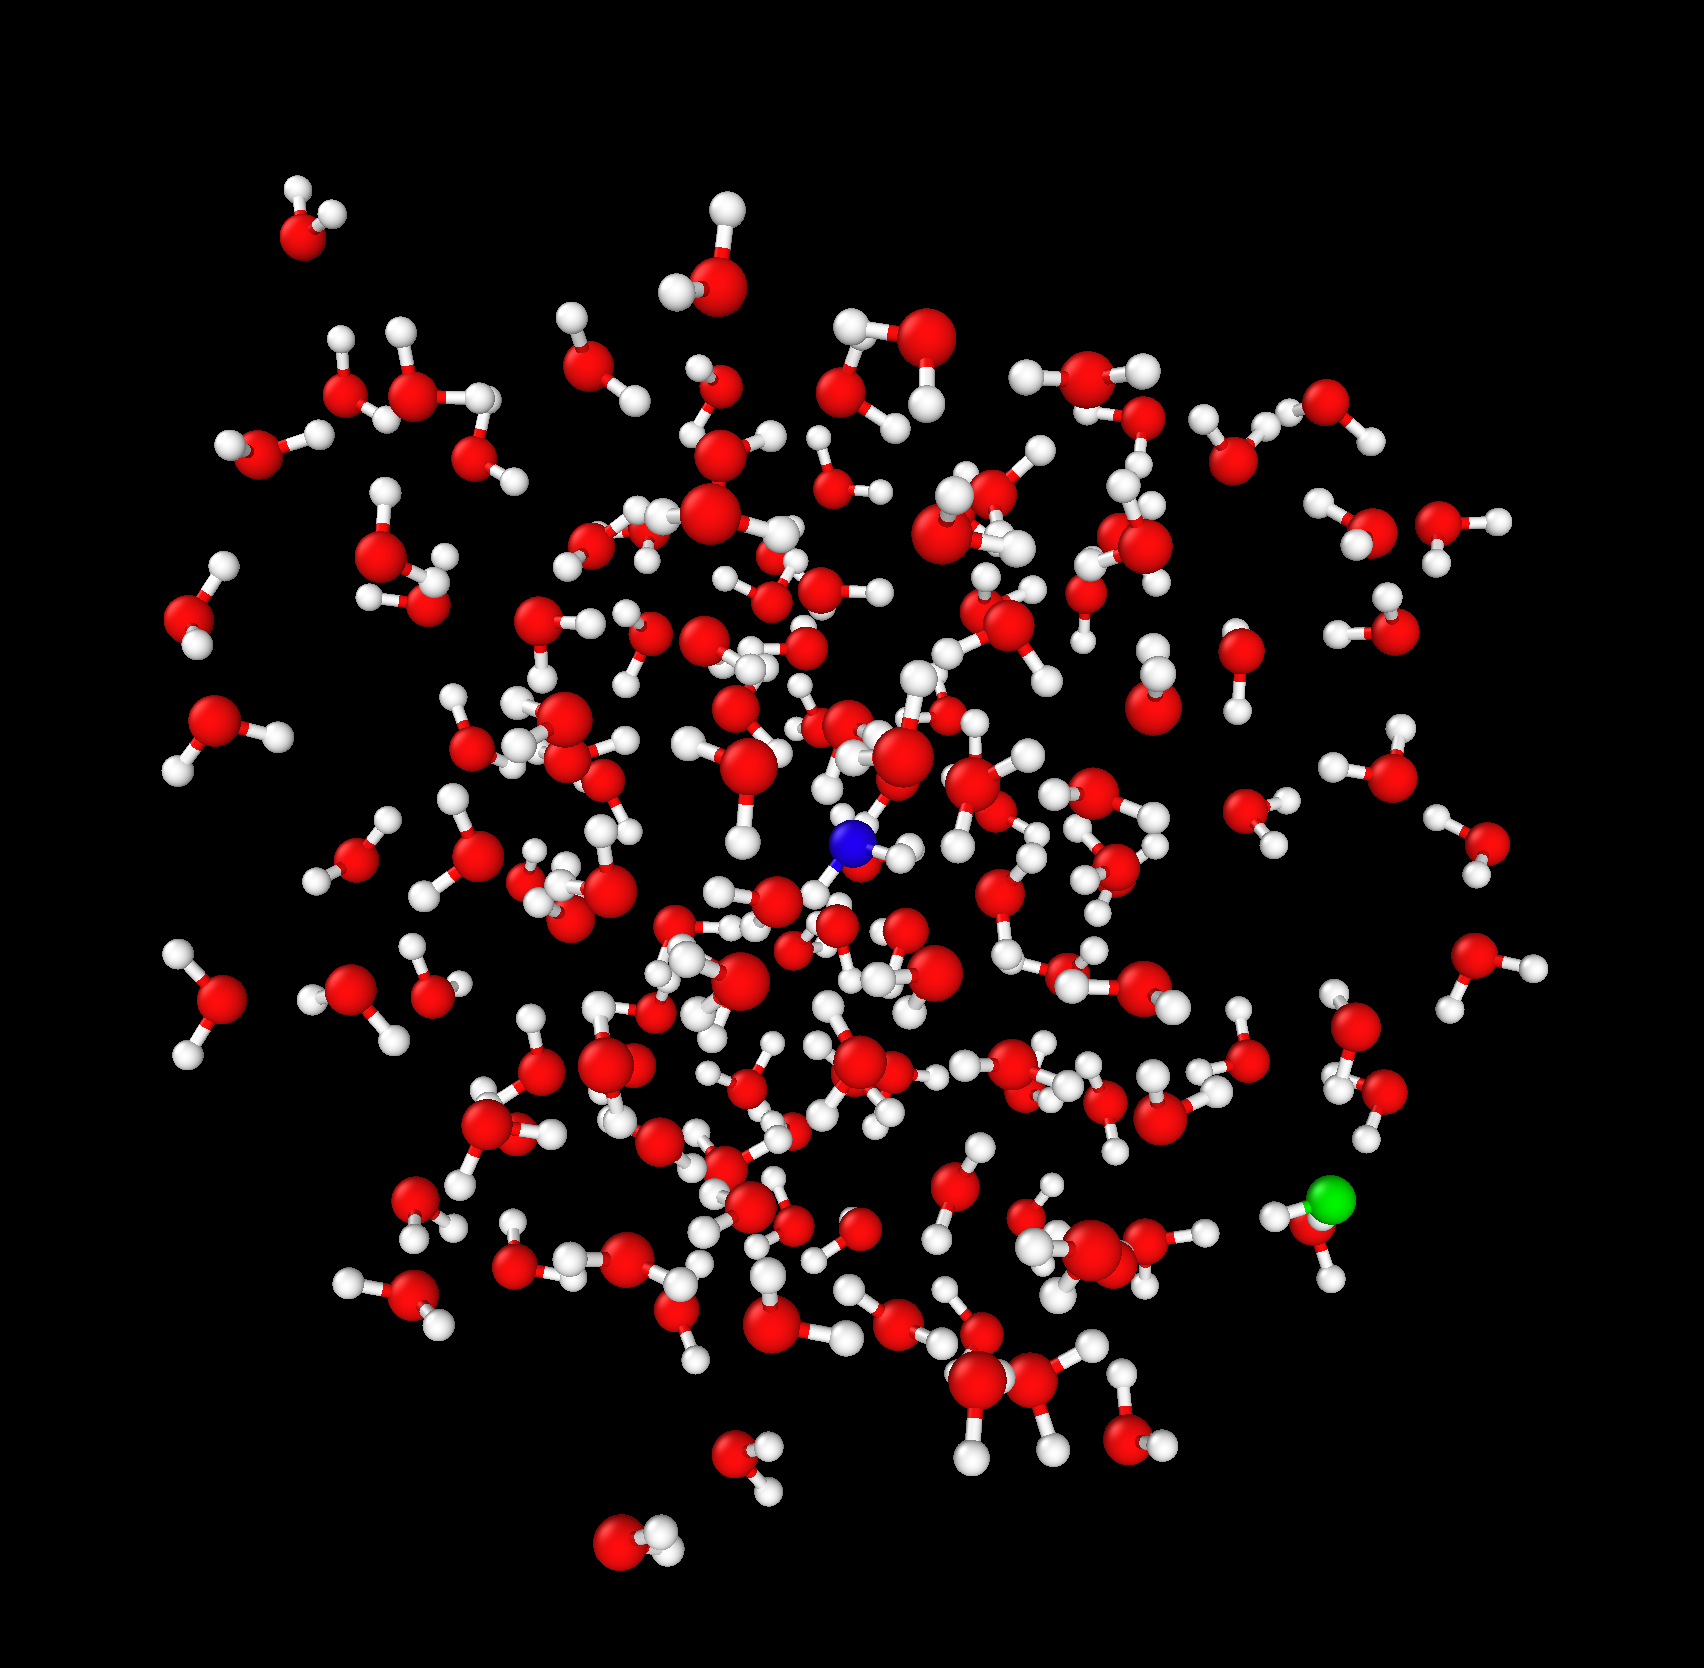
\includegraphics[width=0.8\linewidth]{figures/128}
	\captionof{figure}{\textit{The cell containing 126 water molecules, a hydronium ion and a hydroxide ion. All the hydrogen atoms are coloured white and all the oxygens are coloured red apart from the one that is part of the hydronium ion, which is coloured blue, and the one that is part of the hydroxide ion which is coloured green. This image was created using Ovito. \cite{ovito}}}
	\label{fig:128}	
\end{figure}

\subsection{Self-consistency}
\label{sec:self-consistent}
The tight binding code uses the method described in reference \cite{Paxton2009}. The steps are,
\begin{enumerate}
	\item Solve the eigenproblem for $H^{0}$, the non self consistent Hamiltonian, finding the eigenvector expansion coefficients.
	\item Build the multipole moments and find the components, $V_{\textbf{R}L}$, of the potential.
	\item Assemble the elements of $H'$.
	\item Solve the eigenproblem for $H=H^{0}+H'$.
	\item Repeat until self consistent.
\end{enumerate}

\subsection{Molecular Statics}
\label{sec:relax}
Molecular statics was used to relax our cell to the point where the forces were small enough that the atoms would be stable in molecular dynamics simulations. We used two of the relaxations modes, the Fletcher-Powell algorithm \cite{Fletcher1980,Davidson1959,CTRL} and the Broyden algorithm.\cite{Broyden1965} The former works by finding the minimum energy along a line, changing the line and then updating the Hessian matrix, while the latter is essentially a Newton-Raphson algorithm which updates the Hessian matrix and direction of descent after each step.

We set the XTOL and GTOL tolerances \cite{CTRL} to $10^{-5}$, the number of iterations (NIT) to $10000$ and the distance step (STEP) to between $0.1$ and $0.001$ (using a large step for configurations which relaxed easily, and reducing it where necessary).

\subsection{Molecular Dynamics}
\label{sec:MD}
TBE performs molecular dynamics using the method set out in source \cite{martyna1996explicit}, i.e. using reversible integrators which employ Liouville operators.

In all simulations molecular dynamics was run for a maximum of 10ps with 0.5fs between time steps. NVT mode (which conserves the number of particles, volume and temperature) was used since it was the most stable. The xyz and md files were written to in every frame.

\subsection{Analysis}
By analysing these file, a python script calculated which oxygen atom was part of a hydronium ion in each frame and recorded the temperature. It then calculated the standard deviation in the jumping rate and the temperature. 

By looking at the number of jumps over time we realised that each simulation started with a large number of jumps, before settling in to a steadier, lower rate. This is due to the conditions of the simulations undergoing a sudden change, such that they are less stable for a short time. To compensate for this, we ignored the first 1ps of the simulations. We treated this as a screening period, and only recorded the temperature and jumps following this period.

\section{Results}

\begin{figure}[h]
	\centering
	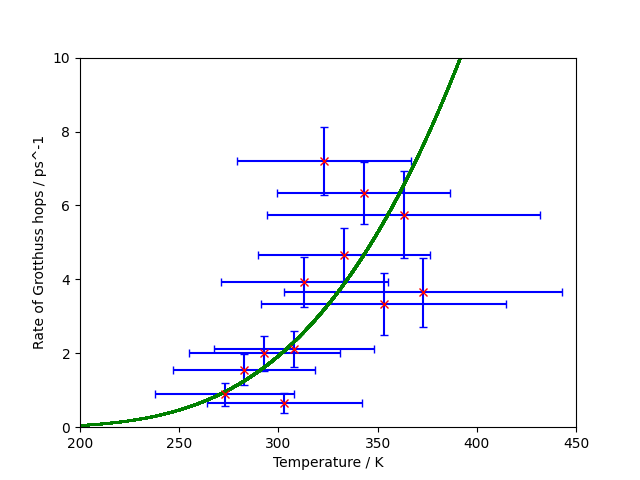
\includegraphics[width=\linewidth]{figures/bestfitcurve.png}
	\caption{\textit{The jumping rate of the hydronium ion in $ps^{-1}$ for a range of temperatures as described in \ref{sec:method} with the first 2000 time steps screened out. A weighted best fit curve is plotted through the data according to equation \ref{eq:arrhenius}.}}
	\label{fig:bestfitcurve}	
\end{figure}
Simulations run at above 350K, which is the upper limit that was used in the paper that this tight binding model was taken from,\cite{Lozovoi2014} had a high likelihood of breaking down in a way that isn’t observed in real water.\cite{bell2013proton} A proton can break away from the hydronium ion if several oxygen atoms come close to it. However in this case, the protons gets suspended in between the water molecules instead of joining one of them to form a new hydronium ion and stays as a lone proton.

To estimate the temperature dependence of the jumping rate we fitted the data to the Arrhenius equation \cite{arrhenius1889dissociationswarme}
\begin{equation}
	\label{eq:arrhenius}
	r = r_{0}\exp{\frac{-E_{A}}{k_{B}T}},
\end{equation}
where $r$ is the jumping rate, $r_0$ is a pre-exponential factor, $E_{A}$ is the activation energy of the reaction and $k_{B}$ is the Boltzmann constant.\cite{planck1900theory}

To find $r_{0}$ and $E_{A}$ we plot $\log r$ against $1/T$ and, using the method set out in reference \cite{gatland1993weight}, we construct a weighted least-squares best fit line and calculated values for $r_{0}$ of $2148.3607\text{ps}^{-1}$ and ${E_{A}}/{k_{B}}$ of $2098.0025$ K.

Returning the axes to linear ones, the data was superimposed on the best fit curve as shown in figure \ref{fig:bestfitcurve}.

Using the Boltzmann constant in eV K$^{-1}$, the activation energy of a Grotthuss jump is calculated as $0.1808\pm 0.0496$ eV and the Grotthuss jumping rate of a hydronium ion in water is 
\begin{equation}
\label{eq:result}
	(2184.36 \pm 509.17)\exp{-\frac{2098.00 \pm 576.81}{T}}.
\end{equation}

\section{Discussion}
The errors in our results are large ($\sigma_{r_{0}}\approx 22\%$ and $\sigma_{E_{A}}\approx 26\%$), however these values do model the process well at most lower temperatures as evidenced in figure \ref{fig:bestfitcurve}, the exception being the anomalously low rate at 303K. This makes a degree of sense as the tight binding model we use, as set out in \cite{Lozovoi2014}, was created only using temperatures between 230K and 350K. Curiously, the three simulations that were run above this temperature range not only broke down, but also had jumping rates below the best fit curve.

However, even though the higher temperature results are not as accurately described by equation \ref{eq:result}, the best fit curve still passes through the error bars of all but one point. This is good evidence that equation \ref{eq:result} is a valid model for the jumping rate in our simulation.
\section{Conclusions}
In conclusion, our tight binding model for water does successfully simulate the Grotthuss process, allowing proton transfer throughout a body of water. 

Our model produces stable molecular dynamics simulations that can last for at least 10ps for temperatures below 350K but breaks down at higher temperatures.

The activation energy of a Grotthuss jump is $0.1808 \pm 0.0496$ eV and the rate at which a proton jumps from on molecule to another is given by the formula $(2184.36 \pm 509.17)\exp{-\frac{2098.00 \pm 576.80}{T}} \text{ps}^{-1}$.


\bibliography{GrotthussBibliography2.bib}
	\bibliographystyle{ieeetr}
\end{document}